\chapter{Conditional Probability and Bayes' Rule}

\section{Conditional Probability}

Let's begin with an example

\begin{eg}
We toss 3 coins. You win if at least two heads come out. What is the probability of winning?

\textbf{Solution:} 
\[
    \Omega = \{\text{HHH}, \text{HHT}, \cdots, \text{TTT}\} \quad\Rightarrow\quad \mathbb{P}(W) = \dfrac{\vert W \vert}{\vert \Omega \vert} = \dfrac{4}{8} = \dfrac{1}{2}
\]
\end{eg}

However, if it is given that the first coin was tossed and came out head. How does this affect your chances of winning? Since the sample space now changes due to the condition that the first toss is heads, the way we find the probability differs. 
\[
    \Omega^{\prime} = \{\text{HHH}, \text{HHT}, \text{HTH}, \text{HTT}\},\quad W^{\prime} = \{\text{HHH}, \text{HHT}, \text{HTH}\}
\]
This give the probability \(\frac{3}{4}\). 

\subsection{Conditional Probability}
\begin{definition}[Conditional Probability]~ 

    \begin{minipage}{0.7\textwidth}
        The Conditional Probability \(\mathbb{P}(A|F)\) represents the probability of event \(A\) assuming (or given) that event \(F\) happened.
    \end{minipage}
    \begin{minipage}{0.3\textwidth}
        \centering
        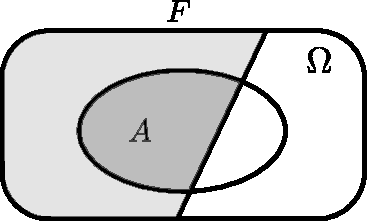
\includegraphics[width=0.7\textwidth]{Figures/ConditionalProbability.pdf}
    \end{minipage}

    \begin{remark}
        All the outcomes of \(\Omega\) and event \(A\) in \(F\) should be excluded in the calculation.
    \end{remark}
\end{definition}

The conditional probability of \(A\) with respect to reduced sample space \(F\) is given by the formula: 
\[
    \mathbb{P}(A|F) = \dfrac{\mathbb{P}(A \cap F)}{\mathbb{P}(F)}
\]

\begin{eg}
    You roll two dice. You win if the sum of the outcomes is 8. If the first die toss is a 4, should you be happy?

    \textbf{Solution:}
    Considering the initial case, we have:
    \[
        \mathbb{P}(W) = \dfrac{\vert W \vert}{\vert \Omega \vert} = \dfrac{5}{36}
    \]
    Let \(D\) be the event that the first toss is a 4. Given \(D\), we have:
    \[
        \mathbb{P}(W|D) = \dfrac{\mathbb{P}(W \cap D)}{\mathbb{P}(D)} = \dfrac{\frac{1}{36}}{\frac{1}{6}} = \dfrac{1}{6}
    \]
    Therefore, the probability of winning increases. 
\end{eg}

\begin{eg}
    For the same game, you win if the sum of the outcomes is 7. The first toss is a 4. Should you be happy?

    \textbf{Solution:} 
    Considering the initial case, we have:
    \[
        \mathbb{P}(W) = \dfrac{\vert W \vert}{\vert \Omega \vert} = \dfrac{6}{36} = \dfrac{1}{6}
    \]
    Let \(D\) be the event that the first toss is a 4. Given \(D\), we have:
    \[
        \mathbb{P}(W|D) = \dfrac{\mathbb{P}(W \cap D)}{\mathbb{P}(D)} = \dfrac{\frac{1}{36}}{\frac{1}{6}} = \dfrac{1}{6}
    \]
    Therefore, the probability does not change. 
\end{eg}

\subsection{Properties of Conditional Probability}
\begin{proposition}[Properties of Conditional Probability]
    Conditional Probability \(\mathbb{P}(\cdot|D)\) are probabilities over reduced sample space \(F\) and satisfy probability axioms:
    \begin{enumerate}
        \item For every \(A\), \(\mathbb{P}(A|F) \geq  0\)
        \item \(\mathbb{P}(F|F) = 1\)
        \item For disjoint events \(A, B\): \(\mathbb{P}(A \cup B|F) = \mathbb{P}(A|F) + \mathbb{P}(B|F)\)    
    \end{enumerate}

    \begin{remark}
        There is no assumption about \(A\) or \(B\) are subsets of \(F\).
    \end{remark}
\end{proposition}

We can then generalize the conditional probability using Uniform Probability Law. Under equally-likely outcomes in \(F\): 
\[
    \mathbb{P}(A|F) = \dfrac{\text{Number of outcomes in}\ A \cap F}{\text{Number of outcomes in}\ F} = \dfrac{\vert A \cap F \vert}{\vert F \vert}
\]

\begin{eg}~ 

    \begin{minipage}{0.7\textwidth}
        There are three cards with Black/Black, Red/Red and Red/Black sides. We randomly draw one card and observe that one of its sides is Black.
    \end{minipage}
    \begin{minipage}{0.3\textwidth}
        \centering
        
\includegraphics[width=0.7\textwidth]{Figures/EgCard.pdf}
    \end{minipage}

    What is the probability that the card's other side is also Black?

    \textbf{Solution:}
    Let \(B\) be the event that the first drawn color is black, and \(E\) be the event that the second drawn color is also black. Then we have:
    \[
        \Omega = \{1F, 1B, 2F, 2B, 3F, 3B\}
    \]
    \[
        \mathbb{P}(E|B) = \dfrac{\vert E \cap B \vert}{\vert B \vert} = \dfrac{2}{3}
    \]
\end{eg}

\subsection{The Multiplication Rule}
\begin{proposition}[The Multiplication Rule]
    For events \(E_1, E_2\) we can write the probability of their intersection \(E_1 \cap E_2\) as 
    \[
        \mathbb{P}(E_1 \cap E_2) = \mathbb{P}(E_1)\mathbb{P}(E_2 \vert E_1)
    \] 
\end{proposition}

In general, for every \(E_1, E_2, \cdots, E_n\), the multiplication rule says 
\[
    \mathbb{P}(E_1 \cap E_2 \cap \cdots \cap E_n) = \mathbb{P}(E_1)\mathbb{P}(E_2 \vert E_1)\mathbb{P}(E_3 \vert E_1 \cap E_2)\cdots\mathbb{P}(E_n \vert E_1 \cap E_2 \cap \cdots \cap E_{n-1} )
\]

\begin{eg}
    A box contains 5 red balls and 15 blue balls. We randomly draw three balls from the box (without replacement). What is the probability that the balls are all red?

    \textbf{Solution:} 
    Let \(R_i\) be the event that the \(i\)-th ball being drawn is red. 
    
    Then we have 
    \[
        \mathbb{P}(R_1 \cap R_2 \cap R_3) = \mathbb{P}(R_1)\mathbb{P}(R_1 \vert R_2)\mathbb{P}(R_3 \vert R_1 \cap R_2) = \dfrac{5}{20} \times \dfrac{4}{19} \times \dfrac{3}{18} = \dfrac{1}{114}
    \]
\end{eg}

\begin{theorem}[Total Probability Theorem]~ 

    \begin{minipage}{0.7\textwidth}
        For every event \(E\) and \(F\) and its complement \(F^c\),
        \[
            \begin{aligned}
                \mathbb{P}(E) &= \mathbb{P}(E \cap F) + \mathbb{P}(E \cap F^c) \\
                &= \mathbb{P}(E \vert F)\mathbb{P}(F) + \mathbb{P}(E \vert F^c)\mathbb{P}(F^c)
            \end{aligned}
        \]
    \end{minipage}
    \begin{minipage}{0.3\textwidth}
        \centering
        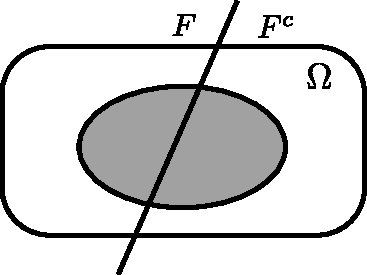
\includegraphics[width=0.7\textwidth]{Figures/TPT.pdf}
    \end{minipage}
\end{theorem}

More generally, if events \(F_1, F_2, \cdots, F_n\) partition \(\Omega\) (disjoint events and \(F_1 \cup F_2 \cup \cdots \cup F_n = \Omega\)), then the total probability theorem says 
\[
    \mathbb{P}(E) = \mathbb{P}(E \vert F_1)\mathbb{P}(F_1) + \mathbb{P}(E \vert F_2)\mathbb{P}(F_2) + \cdots + \mathbb{P}(E \vert F_n)\mathbb{P}(F_n)
\]

\begin{eg}
    A box contains 5 red balls and 15 blue balls. We randomly draw two balls from the box (without replacement). What is the probability that the balls have different colors?

    \textbf{Solution:} 
    Let \(R\) be the event that the first ball is red, \(E\) be the event that the balls have different colors. Then we have 
    \[
        \mathbb{P}(E) = \mathbb{P}(E \vert R)\mathbb{P}(R) + \mathbb{P}(E \vert R^c)\mathbb{P}(R^c) = \dfrac{15}{19} \times \dfrac{5}{20} + \dfrac{5}{19} \times \dfrac{15}{20} = \dfrac{15}{38}
    \]
\end{eg}

\begin{eg}
    For the situation that a group of students answered one multiple choice question where there are 4 options. What is the probability that a student knows the answer to the question?

    \textbf{Solution:} 
    Here we define event \(K\) as student knows the answer to the question, and event \(C\) as student correctly answers the question. Then, the total probability theorem says 
    \[
        \begin{aligned}
            \mathbb{P}(C) &= \mathbb{P}(C \vert K)\mathbb{P}(K) + \mathbb{P}(C \vert K^c)\mathbb{P}(K^c) \\
            &= 1 \times \mathbb{P}(K) + \dfrac{1}{4} \times (1 - \mathbb{P}(K)) \\
            &= \dfrac{3}{4}\mathbb{P}(K) + \dfrac{1}{4}
        \end{aligned}
    \]
    This gives 
    \[
        \mathbb{P}(K) = \dfrac{4\mathbb{P}(C) - 1}{3}
    \]
\end{eg}

\newpage
\section{Bayes' Rule}
We choose a cup at random and then a random ball from that cup. The selected ball is red. Which cup do you guess the ball came from? 
\begin{center}
    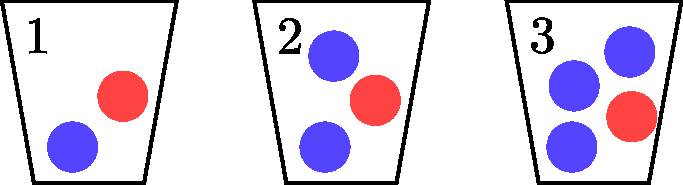
\includegraphics[width=0.3\textwidth]{Figures/EgCup.pdf}
\end{center}
This is an example of cause and effect. Here, the cause is the cup number and the effect is the ball's color. Choosing different cups leads to different probabilities of choosing the color of balls.

\begin{theorem}[Bayes' Rule]
    Consider events \(C\) and \(E\). Then,
    \[
        \mathbb{P}(C \vert E) = \dfrac{\mathbb{P}(E \vert C)\mathbb{P}(C)}{\mathbb{P}(E)} = \dfrac{\mathbb{P}(E \vert C)\mathbb{P}(C)}{\mathbb{P}(E \vert C)\mathbb{P}(C) + \mathbb{P}(E \vert C^c)\mathbb{P}(C^c)}
    \]
\end{theorem}

More generally, if \(C_1, C_2, \cdots, C_n\) partition the set of possible causes \(S\), 
\[
    \mathbb{P}(C_1 \vert E) = \dfrac{\mathbb{P}(E \vert C_1)\mathbb{P}(C_1)}{\mathbb{P}(E \vert C_1)\mathbb{P}(C_1) + \mathbb{P}(E \vert C_2)\mathbb{P}(C_2) + \cdots +\mathbb{P}(E \vert C_n)\mathbb{P}(C_n)}
\]

Let us revisit the example above. Let \(R\) represent the event that a red ball is drawn, and let \(C_i\) denote the cup from which the red ball is drawn, where \(i = 1, 2, 3\). We can then calculate the probability of each cup being the source of the red ball, given that the ball is red.
\[
    \mathbb{P}(C_i \vert R) = \dfrac{\mathbb{P}(R \vert C_i)\mathbb{P}(C_i)}{\mathbb{P}(R \vert C_1)\mathbb{P}(C_1) + \mathbb{P}(R \vert C_2)\mathbb{P}(C_2) +\mathbb{P}(R \vert C_3)\mathbb{P}(C_3)}
\]

For sample space, we have: \(\Omega = \{1B, 1R, 2B_1, 2B_2, 2R, 3B_1, 3B_2, 3B_3, 3R\}\quad (\text{not equally likely}) \)
\begin{table}[H]
    \centering
    \begin{tabular}{c|c|c|c}
        \toprule
             & Cup 1 & Cup 2 & Cup 3   \\
        \midrule
            \(\mathbb{P}(C_i)\)  & \(\frac{1}{3}\)  & \(\frac{1}{3}\) & \(\frac{1}{3}\)  \\[5pt]
            \(\mathbb{P}(R \vert C_i)\)  & \(\frac{1}{2}\) & \(\frac{1}{3}\) & \(\frac{1}{4}\) \\
        \bottomrule
    \end{tabular}
\end{table}

For \(\mathbb{P}(R)\), by using total probability theorem, we have
\[
    \mathbb{P}(R) = \mathbb{P}(R \vert C_1)\mathbb{P}(C_1) + \mathbb{P}(R \vert C_2)\mathbb{P}(C_2) + \mathbb{P}(R \vert C_3)\mathbb{P}(C_3) = \dfrac{1}{2}\times\dfrac{1}{3} + \dfrac{1}{3}\times\dfrac{1}{3} + \dfrac{1}{4}\times\dfrac{1}{3} = \dfrac{13}{36}
\]
Then we have:

\(\mathbb{P}(C_1 \vert R) = \dfrac{\mathbb{P}(R \vert C_1)\mathbb{P}(C_1)}{\mathbb{P}(R)} = \dfrac{\frac{1}{2} \times \frac{1}{3}}{\frac{13}{36}} = \dfrac{6}{13}\), \(\mathbb{P}(C_2 \vert R) = \dfrac{\mathbb{P}(R \vert C_2)\mathbb{P}(C_2)}{\mathbb{P}(R)} = \dfrac{\frac{1}{3} \times \frac{1}{3}}{\frac{13}{36}} = \dfrac{4}{13}\)

\(\mathbb{P}(C_3 \vert R) = \dfrac{\mathbb{P}(R \vert C_3)\mathbb{P}(C_3)}{\mathbb{P}(R)} = \dfrac{\frac{1}{4} \times \frac{1}{3}}{\frac{13}{36}} = \dfrac{3}{13}\)

\begin{eg}
    Two classes take place in the same academic building. Class A has 100 students from whom 20\% are female, Class B has 10 students from whom 80\% are female. 

    Now we see a female student in this building. What is the probability that the student is from Class A? 

    \textbf{Solution:} 
    \[
        \mathbb{P}(A \vert F) = \dfrac{\mathbb{P}(F \vert A)\mathbb{P}(A)}{\mathbb{P}(F \vert A)\mathbb{P}(A) + \mathbb{P}(F \vert B)\mathbb{P}(B)} = \dfrac{20\% \times \frac{10}{11}}{20\% \times \frac{10}{11} + 80\% \times \frac{1}{11}} = \dfrac{5}{7}
    \]
\end{eg}

This example demonstrates a counterintuitive result. Although the proportion of females in Class B is greater than that in Class A, the probability of a female student belonging to Class A is higher. This highlights the importance of using Bayes' rule to update our beliefs, as our initial hypotheses may not always align with the actual probabilities.

To summarize, we see that conditional probability will be a very powerful tool when

1. the studied environment includes causes and effect. This is especially useful for calculating the probability of a cause under an observation of the effect. 

2. we want to calculate an ordinary probability and conditioning on the right event can simplify the description of the sample space. 

\section{Independence}
\subsection{Independence of Two Events}
\begin{definition}[Independent Events]
    We call Events \(A\) and \(B\) independent if 
    \[
        \mathbb{P}(A \cap B) = \mathbb{P}(A)\mathbb{P}(B)\quad\text{or equivalently}\quad  \mathbb{P}(A \vert B) = \mathbb{P}(A)
    \]
\end{definition}

\begin{eg}
    We toss a coin three times. Then the following events are independent: 
    \[
        \Omega = \{\text{HHH}, \text{HHT}, \text{HTH}, \text{HTT}, \text{THH}, \text{THT}, \text{TTH}, \text{TTT}\}
    \]
    Event \(E_1\): The first toss show heads 

    Event \(E_2\): The second and third toss both show tails 
    
    We have: 
    \(\mathbb{P}(E_1) = \frac{4}{8}, \mathbb{P}(E_2) = \frac{2}{8}, \mathbb{P}(E_1 \cap E_2) = \frac{1}{8}, \mathbb{P}(E_1)\mathbb{P}(E_2) = \frac{4}{8} \times \frac{2}{8} = \frac{1}{8} = \mathbb{P}(E_1 \cap E_2)\)

    This shows that the events are independent.
\end{eg}

\begin{eg}
    We roll two dice. Consider events:
    
    \(E_1\): the first die is 4; \(S_6\): the sum of dice is 6; \(S_7\): the sum of dice is 7. 
    \[
    \mathbb{P}(E_1) = \dfrac{1}{6};\ \mathbb{P}(S_6) = \dfrac{5}{36};\ \mathbb{P}(S_7) = \dfrac{1}{6};\ \mathbb{P}(E_1 \cap S_6) = \dfrac{1}{36};\ \mathbb{P}(E_1 \cap S_7) = \dfrac{1}{36};\ \mathbb{P}(S_6 \cap S_7) = 0. 
    \]
    Then we know that (\(E_1, S_6\)) and (\(S_6, S_7\)) are not independent, (\(E_1, S_7\)) are independent.
    \begin{remark}
        Mutually exclusive does not mean independent. 
    \end{remark}
\end{eg}

\begin{proposition}~ 

    \begin{minipage}{0.7\textwidth}
        If \(E, F\) are independent events, then events \(E^c, F\) will also be independent. 
        \[
            \mathbb{P}(E^c \cap F) = \mathbb{P}(E^c)\mathbb{P}(F)
        \]
    \end{minipage}
    \begin{minipage}{0.3\textwidth}
        \centering
        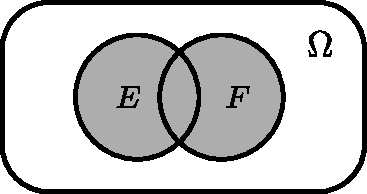
\includegraphics[width=0.7\textwidth]{Figures/PropIndp.pdf}
    \end{minipage}
    
    \begin{proof}
        \[
            \begin{aligned}
                \mathbb{P}(E^c \cap F) &= \mathbb{P}(F) - \mathbb{P}(E \cap F) \\
                &= \mathbb{P}(F) - \mathbb{P}(E)\mathbb{P}(F) \\
                &= \mathbb{P}(F)(1 - \mathbb{P}(E)) \\
                &= \mathbb{P}(E^c)\mathbb{P}(F)
            \end{aligned}
        \]
    \end{proof}
\end{proposition}

\subsection{Independence of Several Events}
We call three events \(A, B, C\) independent events if these four conditions are satisfies:
\begin{enumerate}
    \item \(A\) and \(B\) are independent: \(\mathbb{P}(A \cap B) = \mathbb{P}(A)\mathbb{P}(B)\) 
    \item \(B\) and \(C\) are independent: \(\mathbb{P}(B \cap C) = \mathbb{P}(B)\mathbb{P}(C)\) 
    \item \(A\) and \(C\) are independent: \(\mathbb{P}(A \cap C) = \mathbb{P}(A)\mathbb{P}(C)\) 
    \item And we require \(\mathbb{P}(A \cap B \cap C) = \mathbb{P}(A)\mathbb{P}(B)\mathbb{P}(C)\) 
\end{enumerate}

\begin{eg}
    We roll two dice. Consider events:
    
    \(E_1\): the first die is 4; \(E_2\): the second die is 3; \(S_7\): the sum of dice is 7. 
    \[
    \mathbb{P}(E_1) = \dfrac{1}{6};\ \mathbb{P}(E_2) = \dfrac{1}{6};\ \mathbb{P}(S_7) = \dfrac{1}{6};\ \mathbb{P}(E_1 \cap E_2) = \mathbb{P}(E_1 \cap S_7) = \mathbb{P}(E_2 \cap S_7) = \dfrac{1}{36}.
    \]
    Then we know that (\(E_1, E_2\)), (\(E_1, S_7\)) and (\(E_2, S_7\)) are independent. 
    \[
        \mathbb{P}(E_1 \cap E_2 \cap S_7) = \dfrac{1}{36} \neq \mathbb{P}(E_1) \times \mathbb{P}(E_2) \times \mathbb{P}(S_7)
    \]
    Then we know that (\(E_1, E_2, S_7\)) are not independent. 
\end{eg}

We call \(n\) events \(A_1, A_2, \cdots, A_n\) independent events if for every subset \(\{j_1, j_2, \cdots, j_t\}\) of \(\{A_1, \cdots, A_n\}\), the probability of the intersection is the product of their probabilities:
\[
    \mathbb{P}(A_{j_1} \cap A_{j_2} \cap \cdots \cap A_{j_t}) = \mathbb{P}(A_{j_1})\mathbb{P}(A_{j_2})\cdots\mathbb{P}(A_{j_t})
\]

If \(n\) events \(A_1, A_2, \cdots, A_n\) are independent events, then the independence is preserved when we replace some event(s) by their complements, intersection, unions.

For example, if \(A, B, C, D\) are independent events, then \(A \cup B\) and \(C \cap D\) are also independent events.

\begin{eg}
    Alice wins 60\% of her ping pong matches against Bob. They meet for a 3 match playoff. What are the chances that Alice will win the playoff? 

    \textbf{Solution}
    For Alice, we have
    \[
        \Omega = \{\text{WWW, WWL, WLW, LWW, WLL, LWL, LLW, LLL}\}
    \]
    \[
        A = \{\text{WWW, WWL, WLW, LWW}\}
    \]
    \[
        \mathbb{P}(A) = 0.6^3 + 0.6^2*0.4*3 = \frac{81}{125}
    \]
\end{eg}

\begin{remark}
    One should also be aware that conditioning can affect independence. For example, consider two coins: coin \( A \) with bias \(\mathbb{P}(H \vert \text{coin } A) = 0.9\) and coin \( B \) with bias \(\mathbb{P}(H \vert \text{coin } B) = 0.1\). Suppose we randomly select one of the two coins with equal probability. Then, the probability of getting heads on the 11th toss is:
    \[
    \mathbb{P}(\text{toss 11} = H) = \mathbb{P}(A) \mathbb{P}(H_{11} \vert A) + \mathbb{P}(B) \mathbb{P}(H_{11} \vert B) = 0.5 \times 0.9 + 0.5 \times 0.1 = 0.5.
    \]
    However, if we condition on the event that the first 10 tosses resulted in heads, then it is highly likely that the chosen coin is coin \( A \). In fact, under this condition, we can be certain that we are using coin \( A \). Therefore, the probability of getting heads on the 11th toss given that the first 10 tosses were heads is:
    \[
    \mathbb{P}(\text{toss 11} = H \vert \text{first 10 tosses are heads}) = 0.9.
    \]
\end{remark}

\newpage
\subsection{Conditional Independence}
\begin{definition}[Conditional Independence]
    Events \(A\) and \(B\) are independent conditioned on event \(F\) if
    \[
        \mathbb{P}(A \cap B \vert F) = \mathbb{P}(A \vert F)\mathbb{P}(B \vert F)
    \]
    Note that the above is equivalent to
    \[
        \mathbb{P}(A \vert B \cap F) = \mathbb{P}(A \vert F)
    \]
\end{definition}

\begin{eg}~ 
    \begin{table}[H]
        \centering
        \begin{tabular}{c|c}
            \toprule
                Today & Tomorrow \\
            \midrule
                Sunny & 80\% Sunny, 20\% Rainy \\
                Rainy & 40\% Sunny, 60\% Rainy  \\
            \bottomrule
        \end{tabular}
    \end{table}
    If Today(Monday) is rainy, what is the probability that Wednesday will also be sunny? 

    \textbf{Solution:}
    We suppose weather on Monday and Wednesday are independent conditioned on weather on Tuesday. Let \(M\) be the event that Monday is sunny, same for \(T\) and \(W\). Then: 
    \[
    \begin{aligned}
        \mathbb{P}(W \vert M^c) &= \mathbb{P}(W \vert M^c \cap T)\mathbb{P}(T \vert M^c) + \mathbb{P}(W \vert M^c \cap T^c)\mathbb{P}(T^c \vert M^c) \\
        &= 80\% \times 40\% + 40\% \times 60\% \\
        &= 0.56
    \end{aligned}
    \]
\end{eg}

\begin{eg}[The King's Sibling]
    The king comes from a family of two children. What is the probability that his sibling is female?  

    \textbf{Solution:} Given that the conditions are vague, we need to further set up some conditions for this event.  

    For example, we assume that only boys have precedence. By intuition, it seems the answer is \(\frac{1}{2}\). However, there are 4 possibilities for such an event, including (Boy, Boy), (Boy, Girl), (Girl, Boy), and (Girl, Girl), each with probability \(\frac{1}{4}\).  

    We can ignore the (Girl, Girl) combination since it is stated that there is a king. Then, we have:  
    \[
        \mathbb{P}(\text{Sibling is female}) = \dfrac{\frac{1}{4} \times 2}{\frac{3}{4}} = \dfrac{2}{3}
    \]  

    However, one should note that the probability model we use depends on the conditions we set up or are given. For example, if royal families have different rules on having children, then the probability model would surely be different, leading to different results.  
    
    \begin{remark}
        This example comes from \href{https://ocw.mit.edu/RES-6-012S18}{MIT RES.6-012 Introduction to Probability, Spring 2018}. 
    \end{remark}
\end{eg}

% END OF DOCUMENT